\chapter{Teori}
Dette kapitel har til formål, at give et overordnet indblik i de rum- og psykoakustiske parametre der skal tages højde for ved udviklingen af kunstig binaural lyd i et sæt høretelefoner. 
 
\section{Psykoakustik}

Menneskets øres udformning i både det ydre- mellem- og indre-øre, er anatomisk opbygget til at kunne opfange,forstærke og omsætte lyd fra et fysisk lydtryk til et elektrisk signal i hjernen. Baseret på en række af forskellige praj, også kendt som spatiale cues, kan hjernen lokalisere lydkilden i et rum.
%, så man både kan høre \underline{hvad} det er for en lyd, men også \underline{hvor} lydkilden befinder sig.

Når først det akustiske lydtryk er overført fra luft til væsken i det indre øre, føres vibrationerne igennem øresneglen, som netop står for den første filtrering af signalet, før signalerne sendes videre til hjernen. 
Øresneglens ypperste opgave, er at inddele det indkommende signal, baseret på frekvens, intensitet og timing, før det omformer disse mekaniske vibrationer, til elektriske signaler til hjernen. 
Netop disse tre instanser, er anset som de vigtigste parametre, når man forsøger at 'snyde' øret til at høre i 3D, på trods af at al lyd vil blive udsendt af to enkelte højtalerenheder, placeret lige ved ørets indgang. 
 %Ørerne er designet til at lokalisere lyd i 3 dimensioner, baseret på flere parametre;
 
Hjernens endelige konklusion for en lydkildes lokalisering, kommer ud fra en forskel i menneskets to målepunkter: De to ører. \\
Hjernen kan dermed gestikulere en position ud fra forskellen i ankomsttiden for de to signaler, forskellen i intensitetsniveauet, samt frekvenskarakteristikken for signalet. 

Når man hører en lyd, hører man dog ikke kun den direkte lyd, men også alle de reflektioner der er af lyden, fra det rum, eller de genstande, som lyden passerer undervejs fra sit udspring og til ørerne. 

Hjernen er dog i stand til at registrere hvornår den første lyd ankommer til øret, mens de efterfølgende reflektioner nedprioriteres i vurderingen af lydkildens retning. Dette er kendt som 'the precedence effect'\cite{SpatialBook}, hvor det altså er den første bølgefront som vægtes højest, hvorefter øret henligger efterfølgende, lignende lydsignaler som værende reflektioner. 

Disse reflektioner bidrager til at hjernen kan danne sig et billede af hvilken type rum man står i, men kan ligeledes udgøre en forvirring for hjernen såfremt at rummets efterklangstid er tilstrækkeligt høj. Dette besværliggør netop lokaliseringen af lydkildens origen. 



\section{Interaural Time Difference}

Interaural Time Difference (ITD) er betegnelsen for tidsforskellen fra lyden rammer det første øre, til det rammer det andet øre. Dette cue er særligt hørbart ved frekvenser under 1.5kHz hvor bølgelængden er større end afstanden mellem ørerne på omkring 23cm. 
%, som vist i nedenstående beregning, hvor c er lydens hastighed i luft ved $20^\circ C $.
%
%\( f=1500Hz \hspace{1cm}  c=343\frac{m}{s} \hspace{1cm} t = \frac{1}{f} = 0.6ms  \\ \lambda = t \cdot c = 0.23m \)

Ved disse lavere frekvenser vil afstanden mellem ørerne medvirke en faseforskel i lydsignalet, som bruges til at høre et lille delay imellem de to signaler. Dette delay, benytter hjernen til at beregne en vinkel til lydkilden. Ved højere frekvenser, vil faseforskellen være svær for hjernen at håndtere, da der opnås en form for aliasering af signalet, som det fremgår af figur \ref{fig:AliasITD}.

\figur{.75}{AliasITD}{TV: Begge ører opfanger lyden indenfor samme periode.  \newline  TH: Ørerne opfanger lyden i forskellige perioder.} {AliasITD}

Så længe bølgelængden altså er så tilpas stor, at én periodetid ligger indenfor den forsinkelse, som vil være imellem de to ørers opfattelse af lyden, vil lydkilden altså kunne opleves dominerende fra én retning, som det fremgår af figur \ref{fig:ITD}, hvor kilden er til højre for lytteren. \\
Ved dette eksempel, ses det at lyden ankommer betydeligt før til højre øre, end den gør til det venstre, grundet den længere afstand fra lydkilde til øre.\\
\figur{.5}{ITD}{Illustreret eksempel af kilde-lokalisering ved ITD.\cite{ITDPic}}{ITD}

\section{Interaural Level Difference}
Som den opmærksomme læser måske har bemærket, har lydsignalet i figur \ref{fig:ITD} éns amplitude for begge signaler. Dette skyldes en højere diffraktion af lyden ved de lavere frekvenser, som medvirker en lav dæmpning af lyden, når et mindre objekt som et hoved er 'i vejen' for lydbølgen. \\
I takt med at frekvensen bliver højere, bliver bølgelængden dog mindre og lyden bliver dermed mere direktiv \cite{Elektroakustik}, hvilket medfører en lavere diffraktion omkring hovedet, hvorved der kastes en akustisk skygge som vist på figur \ref{fig:ILD}. \newline
Dette skaber en niveau-forskel imellem de to øres opfattelse af intensiteten af signalet, kendt som Interaural Level Difference (ILD).\\
Hjernen begynder ganske simpelt at bestemme direktiviteten ud fra hvor højt lyden opleves på hvert øre, og baserer dermed en vinkel på den lille forskel der måtte være imellem ørernes niveau. 
\figur{.5}{ILD}{Illustreret eksempel af kilde-lokalisering ved ILD}{ILD}

Som det ses af boksen på ovenstående figur, evalureres der ikke længere på den lille tidsforskel imellem signalerne, men derimod på den øgede amplitude der kan ses for højre øre. Lytteren vil derfor igen opleve lydkilden, som værende mere til højre.

\section{Duplex Teorien}
Netop brugen af ITD og ILD, er gennem historien blev anset som værende de bærende elementer i evnen til at retningsbestemme lydkilder, hvortil overgangen imellem de to elementer blev betegnet af Lord Rayleigh som 'Duplex Teorien', afbilledet i figur \ref{fig:DuplexTeorien}\cite{SpatialBook}.

\begin{figure}[h!]
	\centering
	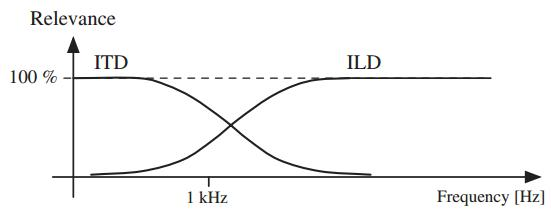
\includegraphics[width=0.7\linewidth]{All_Pics/ITDIID}
	\caption{Prioriteringsgraden af ITD og IID for retningsbestemmelse af et lydobjekt: Duplex Teorien \cite{SpatialBook}}
	\label{fig:DuplexTeorien}
\end{figure}

Som nævnt i tidligere afsnit, ligger overgangen for vægtningen af lyd ved enten ITD eller ILD ved frekvenser på lige over 1 kHz, men det fremgår ligeledes tydeligt at ITD generelt står for lave frekvenser og ILD for de høje.

\section{Begrænsninger for ITD og ILD} 
Alene baseret på ITD og ILD kan det dog være svært at angive præcist hvor en lydkilde befinder sig, da nogle positioner vil kunne opleves ens, indenfor et kegleformet område, som det kan ses på figur \ref{fig:ConeOfConfusion}. Dette skyldes at det akustiske delay og intensiteten af lydsignalet vil have samme værdier, for flere forskellige positioner. 

\figur{.6}{ConeOfConfusion}{Illustration af 'Cone of Confusion'}{ConeOfConfusion}

Fænomenet kaldes "Cone of Confusion", og er et stort problem i gengivelsen af 3D lyd i høretelefoner, som det uddybes i afsnit \ref{sec:3DBasics}. 

I den virkelige verden hviler øret dog ikke alene på disse to cues, men baserer sin evaluering på en lang række cues, såsom reflektioner, lytteoplevelsen i forskellige positioner, synssansen og frekvenskarakteristikkerne som øret genkender for forskellige positioner af lyden. Denne række af cues er dog ikke tilgængelig ved afspilning af lyden i høretelefoner, og man benytter istedet en række konstruerede frekvensspektre-karakteristika: Head Related Transfer Functions.

\section{Head Related Transfer Functions}
\label{sec:HRTF}

Da både ITD og ILD er frekvens-uafhængige elementer for sig selv, er der et behov for flere informationer for en nøjagtigt lokalisering af en lydkilde. Denne kommer fra hjernens genkendelse af positioner ud fra frekvenskarakteristiker, formet af det ydre øre, pinnaen's, udformning. 

Netop reflektioner og diffraktioner, som skabes af torso, hoved og særligt pinnaen, giver nogle særlige dyk og peaks for særlige frekvenser. Igennem de mange år man har benyttet sine ører, har hjernen lært at kategorisere disse særlige kendetegn for diverse frekvenskarakteristikker under specifikke positioner, i særligt det vertikale plan, kaldet elevation.	

Head Related Transfer Function (HRTF) er betegnelsen for denne overføringsfunktion, og udgør den påvirkning som lyden undergår i sin vej fra lydkilden til ørets indgang. Problematikken i HRTF'er består derfor også i den individuelle udformning af Pinnaen hos mennesker. Alle mennesker vil altså opleve lyden med mindre afvigelser i frekvenskarakteristikken, og der er derfor ikke to HRTF-sæt der vil være helt ens. 

For at kunne opnå perfekt 3D-lyd i et par høretelefoner vil der altså være brug for et sæt individuelle HRTF'er for den pågældende testperson, for at personen skulle opleve den konstruerede binaurale lyd som værende ægte. Af samme årsag, vil et generaliseret sæt HRTF'er kunne opleves meget forskelligt under tests. 

\subsection{HRTF i Teorien}
Som tidligere nævnt, udgør en HRTF den påvirkning af et lydsignal som foregår fra lydkilde til lytter. \\
Ved betragtning af lyden i tidsdomænet, bliver HRTF'en til en impulsrespons kalden Head Related Impulse Response (HRIR), som for hvert øres HRIR foldes med det udkommende lydsignal x(t), som det ses i figur \ref{fig:HRTFfoldning}. Dette resulterer i det endelige, spatiale lydsignal $X_L(t)$ og $X_R(t)$.

\figur{.5}{HRTFfoldning}{Foldning af lyden med HRIR}{HRTFfoldning}

Foldningen kan betragtes som i ligning \ref{eq:HRIR}:
\begin{equation}\label{eq:HRIR}
	X_{L/R}(t)=h_{L/R}*x(t)
	\end{equation}
	
	Ved at Fourier-transformere ligningen, opnås der istedet for en foldning, en multiplikation imellem HRIR og lydsignalet, som muliggør en simpel isolering, som det fremgår af ligning \ref{eq:HRTF}:
	\begin{equation}\label{eq:HRTF}
		X_{L/R}(n)=H_{L/R}(n)\cdot X(n) \implies \frac{X_{L/R}(n)}{X(n)}=H_{L/R}(n)
	\end{equation}
	, hvilket indikerer, at såfremt man dividerer det målte signal i lytterpositionen med det afsendte, i frekvens-domæmenet, vil man have en isoleret overføringsfunktion. 
	
	\subsection{HRTF i Praksis}
Mange forskerhold har gennem årene arbejdet med at optage og genskabe HRTF'er for mange forskellige azimuth- og elevation-punkter, ved at måle og optage den impulsrespons som øret oplever, når impulsen opstår i en given azimuth og elevation. Nogle af disse databaser af HRTF'er er blevet standardiseret og samlet under ét, kaldet SOFA (Spatially Oriented Format for Acoustics) \cite{SOFA}. 

Til dette projekt er anvendt databasen fra MIT \cite{MIT} som med 710 målepunkter, dækker elevation fra -40$^\circ$ til 90$^\circ$ i en komplet 360$^\circ$ azimuth i en distance på 1 meter fra en KEMAR som det er vist på figur \ref{fig:mit}.

\figur{.8}{mit}{HRTF målepunkter for MIT KEMAR}{mit}

På figur \ref{fig:hrtfgraf} ses forskellen på en HRTF for hhv højre og venstre øre for en impuls i positionen azimuth = 270$^\circ$ og elevation = 10$^\circ$. Da graferne er skaleret ens er det tydeligt at se, at impulsresponsen for det venstre øre, er væsentligt kraftigere end for det højre øre, og at impulsresponset for det højre øre er mere forsinket end det for det venstre. \footnote{Forskellen i delayet mellem de to impulsresponser er 0.6ms, hvilket svarer til KEMAR'ens hovedstørrelse på 23.4cm}, hvilket altsammen giver mening, da azimuth = 270$^\circ$ er direkte ud for det venstre øre. Kigger man på DFT'en af impulsresponserne ses det også tydeligt, at IID spiller væsentligt ind for det højre øre, hvor de høje frekvenser bliver dæmpet betydeligt pga. hovedets akustiske skygge.

\figur{1}{HRTF_grafer.png}{Fire grafer fra en impuls i positionen azimuth = 270$^\circ$ og elevation = 10$^\circ$. a) Impulsresponsen for højre øre. b) impulsresponsen for venstre øre. c) DFT transformerede impulsrespons for højre øre. d) DFT transformerede impulsrespons for venstre øre. }{hrtfgraf} 
%\fxnote{Forklarende billede af aliasering for ITD? AB}
%For at skabe en digital ITD, sættes et delay mellem hhv højre og venstre signal som svarer til den ønskede azimuth ud fra en fastsat afstand mellem ørerne på 23cm.\fxnote{Hvordan? Hvad er sammenhæng? Beregning? AB}

%\begin{itemize}
%	%\item  Den væsentligste parameter for at kunne identificere et objekt i 3D, er at man har to observationspunkter. I menneskets tilfælde med lyd, har vi et øre placeret på hver side af hovedet, som hver især kan dække en radius af ?? \fxnote{find ud af det - evt i Tores bog LS...Er det en ting? Radius er vel begrænset er kildens lydtryk? AB }. Hvis en lydkilde er placeret væk fra menneskets sagitale\fxnote{Sagitale? AB} plan, vil der være en tidsforskel på, hvornår lyden rammer hvert øre\fxnote{Ved lave frekvenser, AB}. Mere om det i afsnit \ref{sec:ITD}
%
%\item   \fxnote{Noget om T60 ift rumstørrelser og materialer - til efterklangstider LS}
%
%\item  Også det ydre øres udformning, pinneaen, giver forskellige reflektioner\fxnote{overføringskarakteristikker? AB}, alt efter hvorfra lydkilden befinder sig, og ved hjælp af disse individuelle reflektioner, kan hjernen afgøre, hvor lydkilden befinder sig. Mere om dette i afsnit \ref{sec:HRTF}.
%
%
%\end{itemize}
%
%På visse punkter er menneskets hørelse dog også begrænset:
%
%\begin{itemize}
%	\item Ørets frekvensområde ændrer sig over tid. Spædbørn kan høre fra omkring 20Hz - 20kHz, mens en 80-årig måske kun kan høre frekvenser fra 50Hz - 15kHz \fxnote{Find ref LS}. Alle frekvenser bliver heller ikke forstærket lige godt inde i øret. Det vil sige at der skal et relativt større lydtryk til at høre helt dybe eller helt lyse frekvenser, end frekvenser i mellemtoneområdet. Se figur \ref{fig:pressure}
%	
%	\figur{.8}{pressure}{Forholdet mellem SPL og frekvens ved forskellige phon-styrker}{pressure} 
%	
%	\item 
%\end{itemize}